\documentclass[12pt,twoside]{extarticle}
\usepackage[margin=1.2in,top=1.6in,bottom=1.6in]{geometry}
\usepackage[table,dvipsnames]{xcolor}
\usepackage[utf8]{inputenc}
\usepackage{svg}
\usepackage{listingsutf8}
\usepackage{graphicx}
\usepackage{cancel}
\usepackage{empheq}
\usepackage[most]{tcolorbox}
\usepackage{floatrow}
\usepackage[style=numeric,sorting=none]{biblatex}
% \usepackage[spanish,english]{babel}
\usepackage[rightcaption]{sidecap}
\usepackage[bottom]{footmisc}
\usepackage{listings}
\usepackage[T1]{fontenc}
\usepackage{amsmath,amssymb,amsthm}	
% \newtheorem{problem}{Problem}[chapter]
% \newtheorem{definition}{\sffamily Definition}
\usepackage{newtxtext}
\usepackage[varvw]{newtxmath}
\usepackage{esint}
\usepackage[font=small,labelfont=bf,small,sf]{caption}
\usepackage{titlesec}
\usepackage{calc}
\usepackage{fancyhdr}
\usepackage{physics}
\usepackage{hyperref}
\usepackage{lettrine}
% \usepackage{subfig}
\usepackage[cal=cm,scr=boondoxo,bb=px]{mathalfa}
\usepackage{tikz}\usetikzlibrary{shapes.misc}
\usepackage{multicol}
\usepackage{multirow}
\usepackage{booktabs}
\usepackage{subcaption}
\allowdisplaybreaks
\renewcommand{\baselinestretch}{1.2}
\addbibresource{References.bib}
%-------------------------------
%----------- COMANDOS
%-------------------------------
\newcommand{\diff}{\mathrm{d}}
\newcommand{\sol}{\normalfont\textbf{Solution}}
% \renewcommand{\dbar}{d\hspace*{-0.08em}\bar{}\hspace*{0.1em}}
\newcommand{\dem}{\normalfont\bfseries Demostración}
\newcommand{\paren}[1]{\left(#1\right)}
\newcommand{\bracket}[1]{\left[]#1\right]}
\renewcommand{\vector}[1]{\mathbf{#1}}
\newcommand{\unit}[1]{\,\hat{\mathbf{#1}}}
\renewcommand{\r}{\scalebox{0.8}{\rotatebox[origin=c]{335}{$\mathscr{n}$}}}
\newcommand{\bfr}{\scalebox{0.8}{\rotatebox[origin=c]{335}{$\mathbscr{n}$}}}
\newcommand{\ur}{\hat{\bfr}}
\renewcommand{\qedsymbol}{{\color{black!90!white}$\blacksquare$}}
%\newcommand{\eval}{\biggr\rvert}
\renewcommand{\L}{\mathcal{L}}
\newcommand{\barL}{\overline{\L}}
\renewcommand{\v}{\boldsymbol{v}}
\renewcommand{\lstlistingname}{Code}
%---------------------------------
% OPCIONES 
%---------------------------------
\setlength\parindent{20pt}
% \floatsetup[table]{capposition=beside,capbesideposition={right,bottom}}
\arrayrulecolor{black!20!white}
\setcounter{tocdepth}{2}
\setlength\fboxsep{7pt}
\setlength\fboxrule{0.8pt}
\setlength{\headheight}{17pt}
\setlength{\marginparwidth}{2in}
\floatsetup[figure]{capposition=below}
% \newtheorem{theorem}{\bfseries\sffamily Theorem}
\newcounter{theorem}
\newenvironment{theorem}{\stepcounter{theorem}\begin{tcolorbox}[colback=white,colframe=black,enhanced,breakable,sharp corners,boxrule=0.6pt]{\sffamily\textbf{Theorem \thetheorem.}}}{\end{tcolorbox}}
\newcounter{definition}
\newenvironment{definition}[1][]{\stepcounter{definition}\begin{tcolorbox}[colback=black!10!white,colframe=black,enhanced,breakable,sharp corners,boxrule=0.6pt]{\sffamily\textbf{Definition \thedefinition{\,#1}.}}}{\end{tcolorbox}}

\renewcommand{\headrulewidth}{0pt}
\let\arrow\rightarrow
\tcbset{highlight math style={enhanced,
  colframe=black,colback=white,arc=0pt,boxrule=0.5pt,sharp corners}}
\newcommand*{\figref}[2][]{%
  \hyperref[{#2}]{%
    Figure~\ref*{#2}%
    \ifx\\#1\\%
    \else
      \,#1%
    \fi
  }%
}
%---------------------------------
% ENCABEZADO
%---------------------------------
\pagestyle{fancy}
\fancyhead[CO]{\itshape\nouppercase\leftmark}
\fancyhead[RE,RO]{}
\fancyhead[LE,LO]{}
\fancyhead[CE]{\itshape\nouppercase Normal Modes of Oscillation}
\fancyhead[RO,LE]{\bfseries\itshape\thepage}
% \fancyheadoffset[leh,roh]{2.2in}
%---------------------------------
% ------- SECTION DESIGN
%---------------------------------
\titleformat{\section}
  {\normalfont\sffamily\Large\bfseries}{{\sffamily\bfseries\thesection.}}{1ex}{}[{\color{black!20!white}\titlerule[3pt]}]
\titleformat{\subsection}{\sffamily\large\bfseries}{\thesubsection.}{1ex}{}
\titleformat{\subsubsection}{\sffamily\bfseries}{}{0ex}{}
%---------------------------------
% ----------- EXAMPLE
%---------------------------------


%---------------------------------
%-------------- NOTE
%---------------------------------

%------------------------------
% --------- CODE
%------------------------------
\newenvironment{cd}
    {\begin{tcolorbox}[colframe=black!5!white,colback=black!5!white,enhanced,breakable,sharp corners,boxrule=0.6pt]\begin{itemize}\item[]\verbatimfont{\sffamily}}
    {\end{itemize}\end{tcolorbox}}
\newenvironment{code}
    {\verbatimfont{\sffamily}\begin{itemize}\item[]}
    {\end{itemize}}
%---------------------------------
%----- SIGNO DE SUMA CM
%---------------------------------
\DeclareSymbolFont{cmlargesymbols}{OMX}{cmex}{m}{n}
\let\sumop\relax
\DeclareMathSymbol{\sumop}{\mathop}{cmlargesymbols}{"50}
%----------------------------
% LISTING
%----------------------------
\lstdefinestyle{mystyle}{
    backgroundcolor=\color{black!10!white},   
    commentstyle=\color{black!70!white}\sffamily,
    keywordstyle=\color{black}\bfseries\sffamily,
    numberstyle=\sffamily\color{black}\footnotesize,
    stringstyle=\color{black!70!white}\itshape\bfseries\sffamily,
    basicstyle=\sffamily\footnotesize\color{black!70!white},
    breakatwhitespace=false,         
    breaklines=true,                 
    captionpos=b,                    
    keepspaces=true,                 
    numbers=left,                    
    numbersep=10pt,
    showspaces=false,                
    showstringspaces=false,
    showtabs=true,                  
    tabsize=1
}
\lstset{style=mystyle,frame=single}

\makeatletter
% the original definition in amsmath
%\def\intkern@{\mkern-6mu\mathchoice{\mkern-3mu}{}{}{}}
\def\intkern@{\mkern-8mu\mathchoice{\mkern-8mu}{}{}{}}
\makeatother

\makeatletter
\newcommand{\verbatimfont}[1]{\def\verbatim@font{#1}}%
\makeatother

\titlespacing*{\section}{0ex}{2ex}{2ex}
\titlespacing*{\subsection}{0em}{1ex}{0ex}
\titlespacing*{\subsubsection}{0ex}{1ex}{0ex}
\titlespacing*{\paragraph}{0ex}{0ex}{-1ex}
\usepackage{xcolor}
\usepackage{physics}
\usepackage{cellspace}
\usepackage{paracol}% support floats
%------------------------------
% PORTADA
%------------------------------
\title{\bfseries\huge \sffamily Computational modeling of discharging RLC circuits}
\author{\normalfont Freddy Eli Campillo Dorantes}
\date{\itshape\LARGE\bfseries}
\newtheorem{problem}{Problem}
\newcommand{\solution}{{\normalfont\bfseries Solution}}


\begin{document}
\begin{titlepage}
\centering
{\huge\scshape Univesidad de las Américas Puebla \par}
\vspace{0.5cm}
{\Large Department of Actuarial Sciences, Physics and Mathematics\par}
\vspace{2cm}
{
\includegraphics[width=0.4\textwidth]{figures/EscudoUDLAP.jpg}\par}
\vspace{2cm}
{\sffamily\Huge\bfseries Computational moodeling of discharging RLC circuits\par}
\vspace{1cm}
    {\large\itshape Computational Physics Laboratory \par}
\vfill
{\textbf{Autor:}\\
 Freddy Eli Campillo Dorantes\par}
\end{titlepage}
\tableofcontents
\maketitle

\begin{tcolorbox}[colback=black!10!white,colframe=black,enhanced,sharp corners,boxrule=0.6pt]
\begin{abstract}
This report presents the results of a simulation study of RLC circuits with different configurations, including series, parallel, and mixed configurations. The objective of the study was to investigate the frequency and decay rate of each configuration, which are key parameters that determine the circuit's behaviour.

The simulations were carried out using a circuit simulation software, and the results were analysed to determine the circuit's response to different input signals. The frequency and decay rate were calculated using Fourier analysis, which allowed for a detailed characterization of each circuit configuration.

The results show that the frequency and decay rate of the RLC circuits depend strongly on the values of the circuit elements (resistor, inductor, and capacitor) and the configuration of the circuit. The series configuration exhibited a higher natural frequency and slower decay rate compared to the parallel configuration. The mixed configuration showed an intermediate behaviour between the series and parallel configurations.

These findings have important implications for the design and analysis of RLC circuits, as they provide insights into how the circuit's behaviour can be manipulated by varying the circuit parameters and configuration. The results of this study can be used to optimize the performance of RLC circuits in a wide range of applications, including in electronics, power systems, and telecommunications.
 \noindent\textit{Keywords: } RLC circuit, second order circuits, numerical methods, data analysis.
 \end{abstract}
\end{tcolorbox}
\setlength{\parskip}{0.4\baselineskip}\newpage

%----------------------------
% --- Problem Setting
%----------------------------
\section{Introduction}
\subsection{Objectives}
\begin{itemize}\setlength\itemsep{0.25em}
    \item Measurement of the evolution of the current and voltage that characterise the discharging RLC circuit in a parallel and series configurations.
    \item Computational simulation of the tested circuits and comparison of the results with the experimental data.
    \item Obtain and compare the type of solution, as well as the defining parameters, such as natural frequency of the system and the dampening factor.
\end{itemize}

\subsection{The RLC circuit}
\noindent An RLC circuit is an electrical circuit that consists of a resistor, an inductor, and a capacitor connected together. These circuits are used in a wide range of applications, including in electronics, power systems, and telecommunications. In this report, we will explore the behaviour and characteristics of RLC circuits, their applications, and the mathematical models used to describe their behaviour. Understanding the theory behind RLC circuits is essential for designing and analysing more complex electrical systems, and is a fundamental concept in electrical engineering and physics.

An RLC circuit is a type of electrical circuit that includes a resistor (R), an inductor (L), and a capacitor (C) that are connected together. The behaviour of an RLC circuit is governed by the interplay between these three circuit elements. The resistor restricts the flow of current in the circuit, the inductor opposes changes in current by inducing an electromotive force (EMF), and the capacitor stores and releases electrical charge.

These circuits exhibit complex behaviours that can be analysed using complex numbers and second order differential equation. For that reason, these type of circuits are often called second order circuits. In consumer devices, RLC circuits are found in a combination of two basic configurations: series and parallel. These equations describe how the voltage and current in the circuit change over time, and can be solved to predict the circuit's behaviour under different conditions.

%When an RLC circuit is excited with an electrical signal, such as a voltage or a current, it responds with a natural frequency that depends on the values of R, L, and C. The circuit's natural frequency determines how quickly it can transfer energy between the inductor and the capacitor, and is a key parameter in the circuit's behaviour.
In this report, discharging RLC circuits will be covered. This means that no voltage source will be used. Given that the circuit is closed and the capacitor has stored energy in the form of electric charge, $t$ is the time elapsed since the switch was closed, $R$ is the resistance, $L$ the inductance,  and $C$ is the capacitance. As time elapses the capacitor starts to discharge, the energy stored in the capacitor is dissipated as heat in the resistor and magnetic energy in the inductor. Depending on the configuration and the specific values of the three former parameters, the circuit can exhibit three different behaviours: \textit{underdamped}, \textit{critically damped}, and \textit{overdamped}.

Each of these classifications correspond to a behaviour similar to known functions:
\begin{itemize}\setlength\itemsep{0.25em}
    \item  The underdamped configurations behaves to a decaying sine function. That is, of the form 
        \begin{equation} U(t)=Ae^{-\alpha  \sin \qty(\omega t + \phi)}.\end{equation}
    \item  The critically damped configurations behaves just like an exponential function. That is, of the form 
        \begin{equation} C(t)=Ae^{\alpha}.\end{equation}
    \item  The overdamped configurations behaves like a linear combination of exponentials. That is, of the form 
        \begin{equation} O(t)=Ae^{\alpha}+Be^{\beta} .\end{equation}
\end{itemize}

In order to figure which of the three pattern we can expect of a circuit, we must first determine de configuration of the components. As stated before, we are only concerned for the \textit{series} and \textit{parallel} cases.
\subsubsection{RLC in series}

\begin{figure}[ht]
    \centering
    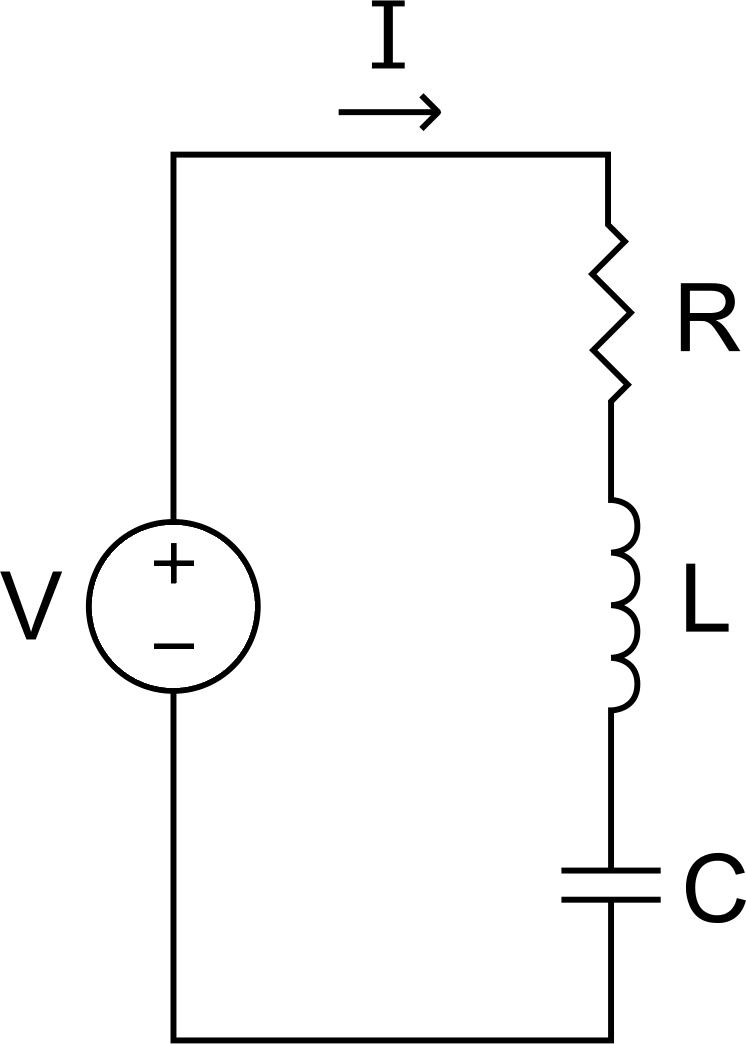
\includegraphics[width=0.35\columnwidth]{figures/RLC_series.png}
    \caption{An example RLC circuit in a series configuration without a voltage source.}
    \label{fig:seriesRLC}
\end{figure}
According to \cite{bobrow1983analisis}, in order to analyse an RLC circuit in a series configuration given the initial conditions for the voltage ($v_0$) and the current ($I_0$) in the capacitor, one must use Kirchoff's first law  to find the following equation:
\begin{equation}
    L\dv{i}{t} + Ri + \frac{1}{C} \int_{-\infty}^t i \dd{t}
\end{equation}
This differential equation governs the discharging behaviour of the circuit, where $i$ is the current flowing through the circuit at time $t$, $L$ is the inductance, $R$ is the resistance, and $C$ is the capacitance. From here, it is convenient to center the analysis only on the capacitor, as the equation that describes it,
\begin{equation}\label{eq:cap}
    i=C\dv{v}{t},
\end{equation}
is useful to obtain the following equation.
\begin{equation}
    \dv[2]{v}{t}+\frac{R}{L}\dv{v}{t} + \frac{1}{LC} = 0.
\end{equation}
It is here when we have two define two new parameters, $\alpha$ and $\omega_n$, that will indicate the behaviour of the circuit.
\begin{equation}
    \alpha = \frac{R}{2L}, \,\,\,\,\,
    \omega_n = \frac{1}{\sqrt{LC}}.
\end{equation}

\begin{itemize}\setlength\itemsep{0.25em}
    \item  If $\alpha$ <$\omega_n$, then the system is underdamped, and the voltage is given by:
        \begin{equation} V_u(t)=Ae^{-\alpha  \sin \qty(\omega_d t + \phi)}.\end{equation}. 
        where $\omega_d = \sqrt{\omega_n^2-\alpha^2}$, and both $A$ and $\phi$ are set by the initial conditions.
    \item  The critically damped configurations behaves just like an exponential function. That is, of the form 
        \begin{equation} V_c(t)=Ae^{\alpha}.\end{equation}
        where $A$ is set by the initial conditions.
    \item  The overdamped configurations behaves like a linear combination of exponentials. That is, of the form 
        \begin{equation} V_o(t)=Ae^{s_1}+Be^{s_2} .\end{equation}
        where $s_{1,2} =-\alpha\pm \sqrt{\omega_n^2-\alpha^2}$, and both $A$ and $B$ are set by the initial conditions.
\end{itemize}

In all of the above scenarios, one can find the function of the current by differentiation of that of the voltage, according to equation \ref{eq:cap}.

\subsubsection{RLC circuits in parallel}
For the parallel configuration, it is more suitable to describe the evolution of the current in the inductor. Remembering that the equation that describes an ideal inductor is the following,
\begin{equation}\label{eq:induc}
    V = L \dv{i}{t}
\end{equation}
And given the same initial conditions and parameters that were used in the previous example, by using the same methodology, one can find the equation that characterises the parallel RLC circuit.
\begin{equation}
    \dv[2]{i}{t} + \frac{1}{RC}\dv{i}{t} +\frac{1}{LC}{i}
\end{equation}
\begin{figure}[ht]
    \centering
    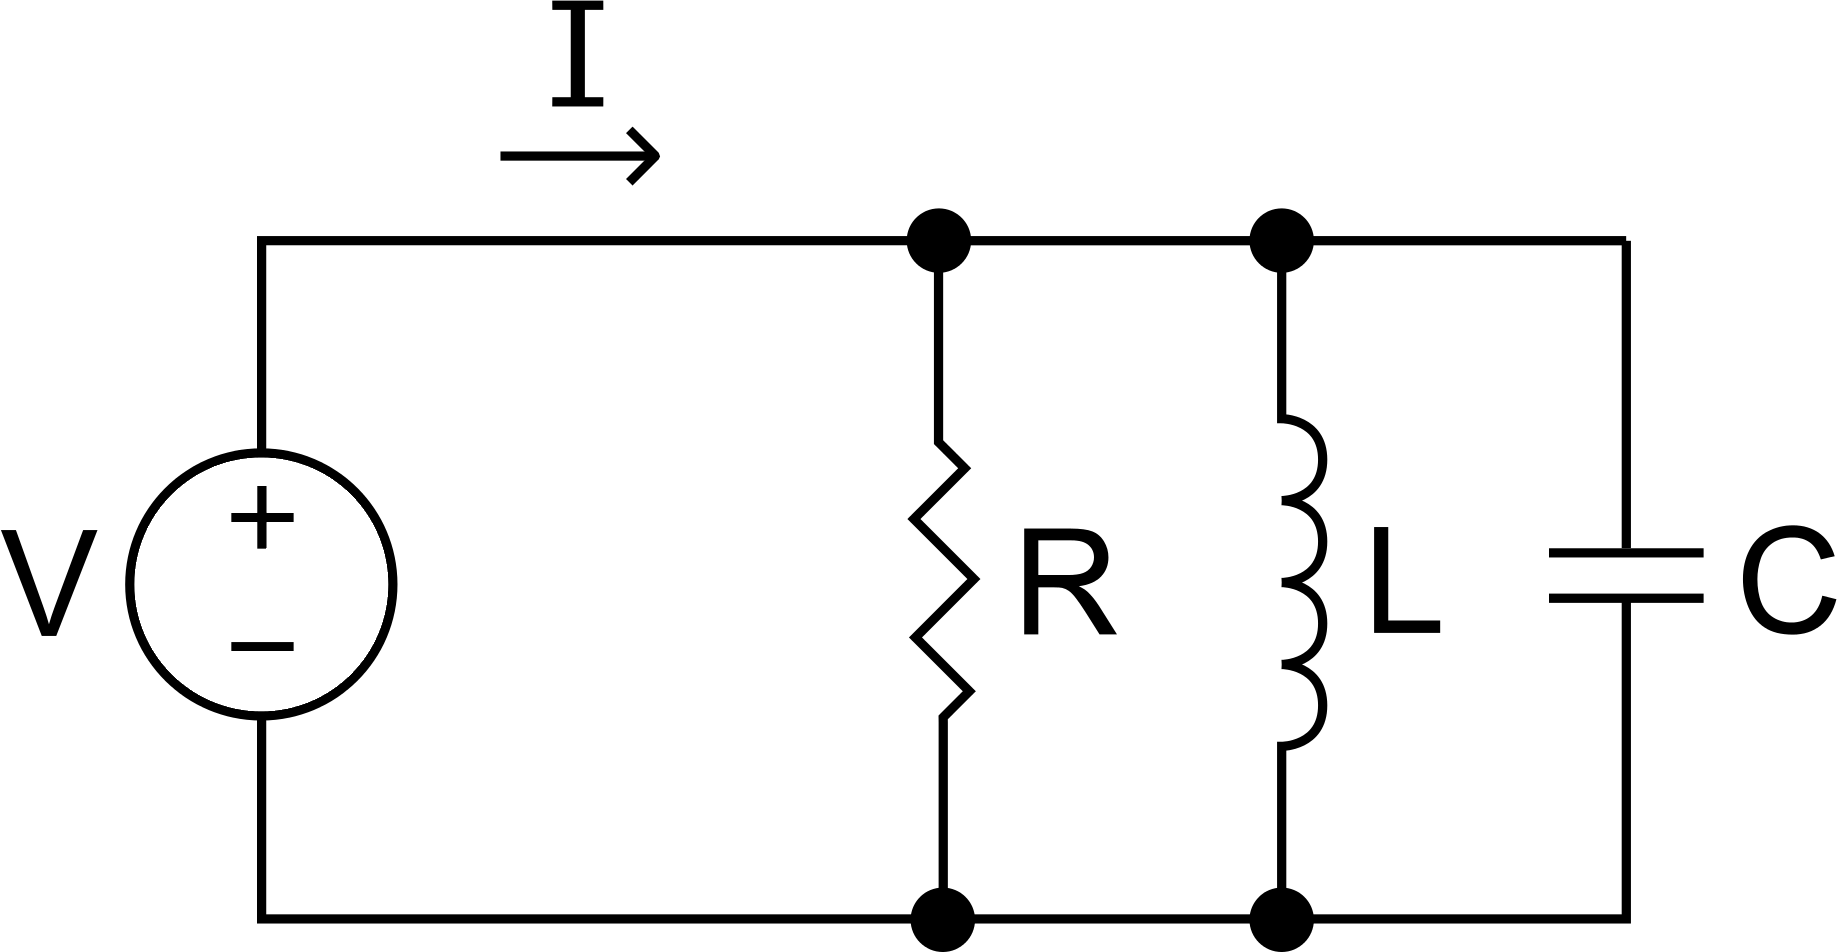
\includegraphics[width=0.6\columnwidth]{figures/RLC_parallel.png}
    \caption{An example RLC circuit in a parallel configuration without a voltage source.}
    \label{fig:parallelRLC}
\end{figure}
With this new differential equation, the parameters $\alpha$ must be redefined as,
\begin{equation}
    \alpha = \frac{1}{2RC},
\end{equation}
while the rest of the definitions and classifications remain the same as the series configuration, with the exception that now the function represents the current instead of the voltage. The later can be calculated by differentiation, as stated in equation \ref{eq:induc}.

\subsection{The Runge-Kutta 4 method}
%\noindent The Runge-Kutta 4 method is a numerical algorithm used to solve ordinary differential equations (ODEs) by approximating the solution at discrete time steps. The method is a fourth-order, explicit method, meaning that it uses information at the current time step and previous time steps to estimate the solution at the next time step.
%
%The basic idea behind the Runge-Kutta 4 method is to estimate the derivative of the solution at four different points within the time step, and then use a weighted average of these estimates to compute the approximate solution at the end of the time step. This weighted average is called the Runge-Kutta formula, and is calculated using a set of coefficients that depend on the order of the method.
%
%The Runge-Kutta 4 method is widely used because it provides a good balance between accuracy and computational efficiency. It is more accurate than lower-order methods such as the Euler method, and can be used to solve a wide range of ODEs with relatively small time steps.
%
%To use the Runge-Kutta 4 method, the ODE must first be converted to a system of first-order ODEs. The method then proceeds by iterating through the time steps, using the Runge-Kutta formula to estimate the solution at each time step. The accuracy of the method can be improved by decreasing the size of the time step, although this can come at the cost of increased computational complexity.
%
%Overall, the Runge-Kutta 4 method is a powerful tool for solving ODEs numerically, and is widely used in a variety of fields, including physics, engineering, and computer science.

Following  Burden 2015 \cite{burden2015numerical} we'll first give and introduction to the Runge-Kuta method of order 4 for a single first order equation, then we'll briefly introduce how to reduce a second order equation to two first order equations to finally introduce the Runge-Kuta method of order 4 for a system of six first order equations.

\subsubsection{Runge-Kutta method of order 4}
    Recall that a first order differential equation has the form:
    \begin{align*}
        y'=f(t,y), \quad \text{for} \quad a \leq t \leq b, \quad \text{subject to} \quad y(a)=\alpha
    \end{align*}
    And recall that,
    supposing that this initial value problem (IVP) is well posed, we will be able to use the Runge-Kutta method of order four to approximate the solution $y$ in this interval.
    
    First we will need to pick a number of $n+1$ equally spaced points in the interval $[a,b]$ in order to define the step size $h>0$, the initial $t_0$ and the starting value $y_0$ as:
    \begin{align*}
        h&=\dfrac{b-a}{n} \\
        t_0 &= a \\
        y_0 &= y(a)=\alpha
    \end{align*}
    This now defines in which points of the interval we'll be approximating the function. This points are defined as:
    \begin{align}
        t_{n+1}=t_n + h \quad \lor \quad t_{n+1} = t_0 +nh = a +nh
    \end{align}
    Now we need to compute what is pretty much the essence of this method, the $ki$'s coefficients, defined as:
    \begin{align*}
        k_1&=hf(t_n,y_n) \\
        k_2&=hf\hspace{0.1em} \left(t_n+\dfrac{h}{2}, y_n + \dfrac{k_1}{2}\right)\\
        k_3&=hf\hspace{0.1em} \left(t_n+\dfrac{h}{2}, y_n + \dfrac{k_2}{2}\right)\\
        k_4&=hf\hspace{0.1em} \left(t_n+h, y_n + k_3\right)
    \end{align*}
    Note that this computations are actually values of the function $f$, which we may also interpret as slopes of $y$, on different parts of the interval between $t_n$ and $t_{n+1}$. Note that $k_1$ is the slope of $y$ at the beginning of the interval, $k_2$ is the slope at the midpoint of the interval but with $k_1$, $k_3$ is also the value of $y$ in the midpoint but now with $k_2$, and $k_4$ is the slope at the end of the interval using $k_3$ and so, for each interval we get values of how the function behaves, we now define the approximation on this interval with a weighted average as:
    \begin{align*}
        y_{n+1}=y_n + \dfrac{1}{6}\Big(k_1+2k_2+2k_3+k_4\Big)
    \end{align*}
    These are the ideas of this method and should not be mistaken as either a pseudocode or an algorithm. It's important to say that this method has a local truncation error $O(h^4)$ provided that the solution $y$ has five continuous derivatives i.e. $y\in C^5$.
    
\subsubsection{Second Order Differential Equations}
    Consider the following second order IVP problem:
    \begin{align*}
        y''=f(t,y,y'), \quad \text{for} \quad a \leq t \leq b, \quad \text{subject to} \quad y(a)=\alpha_1, \ y'(a)=\alpha_2
    \end{align*}
    To attack this kind of problem we can reduce the second order IVP into a system of 2 first order
    equations. We do this basically by re-naming variables. By assigning the labels $u_1(t)=y(t)$, $u_2(t)=y'(t)$ we get the following system:
    \begin{align*}
        \begin{aligned}%[center]
            \dot{u}_1 &= u_2 \\
            \dot{u_2} &= f(t,u_1,u_2) \\
        \end{aligned}
        \quad\quad
        \begin{aligned}%[center]
            u_1(a) &= \alpha_1 \\
            u_2(a) &= \alpha_2 
        \end{aligned}
    \end{align*}
    Making a problem with an unknown solution into a solvable problem.

\subsubsection{Runge-Kutta method for a system of 2 first order ODE's}
Now we'll give the algorithm of the RK4 method for a IVP system of 2 first order ODE's. 

Consider a first order IVP system of 2 equations with the form:
\begin{align*}
    u'_j=f_j(t,u_1,u_2), \quad a \leq t \leq b, \quad \text{with} \quad u_j(a)=\alpha_j
\end{align*}

for $j=1,2$ at $n+1$ equally spaced points in the interval $[a,b]$:\par

\begin{itemize}
    \item[{\bf IN}] endpoints $a$, $b$; integer $n$, initial conditions $\alpha_1$, $\alpha_2$.
    
    \item[ {\bf OUT}] approximations $w_j$ to $u_j(t)$ at the $n+1$ values of $t$. 
    \item[Step 1]
    set $h=(b-a)/n$; \\
    \indent\hspace{0.4cm} t=a.
    
    \item [Step 2]
    For $j=1, 2$ set $w_j=\alpha_j$
    
    \item[Step 3]
    \textbf{OUT} $(t, w_1, w_2)$
    
    \item[Step 4]
    For $i=1,...,n$ do steps 5-11 .
    
        \subitem Step 5 For $j=1, 2$ set \\
        \indent\hspace{2.3cm} $k_{1,j}=hf_j(t,w_1,w_2)$
        
        \subitem Step 6 For $j = 1, 2$ set \\
        \indent\hspace{2.3cm} $k_{2,j}=hf_j \left(t+\dfrac{h}{2},w_1+\dfrac{1}{2}k_{1,1}, w_w+\dfrac{1}{2}k_{1,w}\right)$
        
        \subitem Step 7 For $j = 1, 2$ set \\
        \indent\hspace{2.3cm} $k_{3,j}=hf_j \left(t+\dfrac{h}{2},w_1+\dfrac{1}{2}k_{2,1}, w_2 +\dfrac{1}{2}k_{2,2}\right)$
        
        \subitem Step 8 For $j = 1, 2$ set \\
        \indent\hspace{2.3cm} $k_{4,j}=hf_j \left(t+\dfrac{h}{2},w_1+\dfrac{1}{2}k_{3,1}, w_2+\dfrac{1}{2}k_{3,2}\right)$
        
        \subitem Step 9 For $j = 1, 2$ set \\
        \indent\hspace{2.3cm} $w_j = w_j + \dfrac{1}{6}\qty\Bigg(k_{1,j} + 2k_{2,j} + 2k_{3,j} + k_{4,j})$
        
        \subitem Step 10 Set $t=a + ih$
        
        \subitem {\bf OUT} $(t, w_1, w_2)$.
    
    \item[Step 12] STOP
\end{itemize}

\subsection{Parameter calculations}
Once the functions of the voltage and current are obtained, either numerically or experimentally; we would like to have a reliable way to compare our solutions with their analytical counterpart. One method can be to calculate some variation of the mean error or percent error of the samples; but, since we know the form the function will adopt, just with a few parameters yet to be defined, we can instead calculate these parameters for each dataset and compare how well they resemble each other.

This is a simple optimisation problem that can be solved by the least squares method.
\subsection{Least squares}
The least squares method is a mathematical technique used to find the best-fit curve (usually a polynomial) that describes the relationship between two or more variables. It is commonly used in regression analysis to determine the relationship between a dependent variable and one or more independent variables.

The basic idea behind the least squares method is to minimize the sum of the squared differences between the observed data points and the predicted values of the dependent variable based on the independent variable(s). In other words, the method seeks to find the function that minimizes the sum of the squared errors between the predicted values and the actual observed values.

\begin{equation}
    y = f(x;\beta) + \epsilon
\end{equation}

\begin{equation}
    r_i = y_i - f(x_i;\beta)
\end{equation}

\begin{equation}
    S= \sum_i r^2_i,  \,\,\,\,\, \min_\beta S
\end{equation}
Finding the minimum of the above function is as simple as equation the gradient to zero.
\begin{equation}
    \grad_\beta S=0
\end{equation}
The problem ends up reducing to solving a matrix problem since
\begin{equation}\label{eq:min}
    \pdv{S}{\beta_j} = 2\sum_i r_i \pdv{r_i}{\beta_j}= -2\sum_i \pdv{f(x;\beta)}{\beta_j}=0,\,\,\,\, j=1,...,m 
\end{equation}

\subsubsection{Non-linear problem}
As we know the type of functions we will be dealing with, we know that they will not be linear. This difficult the parameter calculations since the derivative needed in equation \ref{eq:min} would not necessarily be linear, meaning we could not construct the expected matrix to solve the problem.

\begin{equation}
    L= \sum_i r^2_i,  \,\,\,\,\, \min_\beta L, \,\,\,\,\, f(x;\beta) \neq x^T \beta
\end{equation}
This new problem cannot be solved by regular least squares theory. The solution must be approximated, using an initial guess for the array of parameters and improving on it with the next iteration.
We can use even the simplest root finding algorithm, the Newton-Raphson's method:
\begin{equation}
    x_{i+1}= x_i - \frac{f(x_i)}{f'(x_i)}
\end{equation}
Nevertheless, since we want to find the root of the derivative of a function and not the function itself, we must modify the algorithm a bit, changing the function for its derivative and the derivative for the second derivative, as follows.
\begin{equation}
    x_{i+1}= x_i - \frac{f'(x_i)}{f''(x_i)}
    = x_i -(\laplacian_x f)^{-1} \grad_x f
\end{equation}

This, in essence, implies the calculation of the Hessian, which can be a complicated process, so it if often approximated. Given that we can express the gradient in terms of the Jacobian matrix,
\begin{equation}
    \nabla_{\beta_j} S = \sum_i 2r_i \cdot \pdv{r_i}{\beta_j}
    =-2\sum_i r_i \cdot \pdv{f_i}{\beta_j} = -2\cdot J^T \cdot r
\end{equation}
where,
\begin{equation}
    J=
    \mqty(\pdv{f_1}{\beta_1} & \hdots &\pdv{f_1}{\beta_p}\\
    \vdots & \ddots & \vdots \\
    \pdv{f_n}{\beta_1} & \cdots & d\pdv{f_n}{\beta_p}), 
\,\,\,\,\,  
\,\,\,\,\,  
    r = \mqty( r_1\\ \vdots \\ r_n).
\end{equation}

Then we can also express the Hessian only with the Jacobian, assuming that the cross derivatives as negligible small.
\begin{equation}
    \laplacian_{\beta_j\beta_k} L = -2 \sum_i \qty(- \pdv{f_i}{\beta_k}\cdot \pdv{f_i}{\beta_j} + \cancel{ r_j \pdv{f_i}{\beta_j}{\beta_k}})  \approx \sum_i \pdv{f_i}{\beta_k}\pdv{f_i}{\beta_j} = 2\cdot J^T\cdot J
\end{equation}

With the above equations, we can create an iterative method to obtain the needed parameters.

\begin{equation}
    \beta_{t+1}= \beta_t - \qty(\laplacian_\beta L)^{-1} \nabla_\beta L \approx \beta_t - \qty(2\cdot J_t^T\cdot J_t)^{-1}\qty(-2 \cdot J^T_t \cdot r_t)
\end{equation}


\begin{equation}
    \boxed{
    \beta_{t+1} \approxeq \beta_t + \qty(J_t^T\cdot J_t)^{-1}\qty(\cdot J^T_t \cdot r_t)
    }
\end{equation}

%%%%%%%%%%%%%%%%%%%%%%%%%%%%%
%% Numerical methodology
%%%%%%%%%%%%%%%%%%%%%%%%%%%%%
\section{Methodology}
\subsection{Circuit}
To measure the voltage and current of an RLC circuit in both series and parallel configurations, the following methodology can be used:

Prepare the RLC circuit by connecting the components in the desired configuration (series or parallel).

Power on the circuit and wait for it to reach a steady-state.

Use a multimeter to measure the voltage across the resistor (Vr), capacitor (Vc), and inductor (VL) in the circuit. To measure the voltage in parallel, connect the multimeter in parallel with the component being measured. To measure the voltage in series, connect the multimeter in series with the component being measured.

Use a second multimeter to measure the current flowing through the circuit. To measure the current in series, connect the multimeter in series with the circuit. To measure the current in parallel, connect the multimeter in parallel with the circuit.

Record the voltage and current measurements in a table, along with any relevant information about the circuit configuration and component values.

Repeat steps 3-5 for different values of the frequency or other relevant variables, to observe changes in the behavior of the circuit.

Analyze the data to calculate the impedance of the circuit, using the equation Z = V/I, where Z is the impedance, V is the voltage, and I is the current. For series circuits, the impedance is equal to the sum of the resistance, inductive reactance, and capacitive reactance. For parallel circuits, the impedance is equal to the reciprocal of the sum of the reciprocals of the resistance, inductive reactance, and capacitive reactance.

Plot the data on a graph to visualize the behavior of the circuit, and compare the results for different circuit configurations and component values.

Overall, the methodology for measuring the voltage and current of an RLC circuit involves using multimeters to measure the voltage and current, recording the measurements, and analyzing the data to calculate the impedance and visualize the behavior of the circuit.

\subsection{Simulation}
To perform computational simulation of RLC circuits, the following methodology can be used:

Choose a suitable software package for simulating RLC circuits, such as LTspice, Multisim, or PSpice.

Create a circuit schematic using the software, with the components arranged in the desired configuration (series or parallel).

Assign appropriate values for the resistance, inductance, and capacitance of the components in the circuit.

Set up the simulation parameters, such as the time step and simulation time.

Run the simulation and collect data on the voltage and current at various points in the circuit, as well as other relevant parameters such as power dissipation and frequency response.

Analyze the simulation data using software tools, such as MATLAB or Python, to calculate the impedance of the circuit and visualize the behavior of the circuit.

Compare the results of the simulation with theoretical calculations, to validate the accuracy of the simulation.

Perform sensitivity analysis by varying the values of the components in the circuit to observe how changes affect the behavior of the circuit.

Document the simulation results and include them in the report, along with relevant graphs and tables.

Overall, the methodology for simulating RLC circuits involves creating a circuit schematic, assigning component values, running a simulation, analyzing the data, and validating the results. By using software tools to simulate RLC circuits, it is possible to study the behavior of circuits under different conditions and to gain a deeper understanding of their characteristics.


\section{Results}
The computational code, given in the apprendix section, produced an output file that contains the evolution of the current and voltage through a specific component of the circuit, given that the voltage between and current passing through any given point in the circuits can be calculated with simple arithmetic calculations based on the values of the resistant inductance or capacitance of the components. For that reason, only one function is needed for characterising the whole configuration.

In order to verify the validity of the simulation a comparison with other two functions was decided: an analytic method and an experimental one. The analytic method is the solution given in previous sections, meanwhile the experimental one is the real live measurements given by replicating the circuits. 

For the serires circuit the voltage and current for the capacitor in the circuit was found. As for the values of the components that were used, it is clear that we are dealing with an underdemped behaviour, meanin the function is expected to be of the form of equation \label{eq:decayingsine}.   

\begin{figure}[ht]
    \centering
    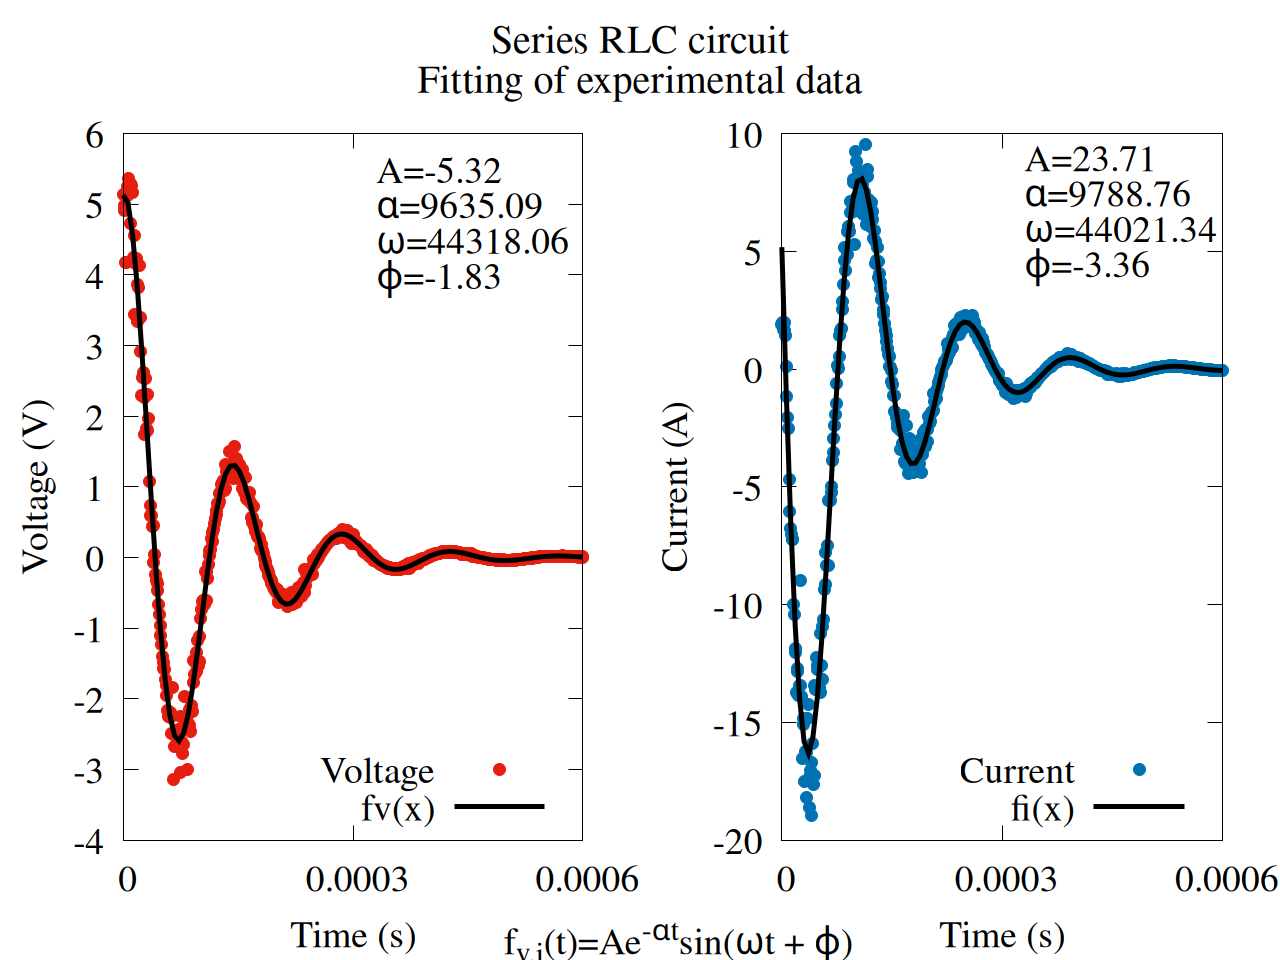
\includegraphics[width=0.9\textwidth]{figures/series_exp_vs_fitting.png}
    \caption{Experimental data and fitting for the series RLC circuit.}
    \label{fig:series_evf}
\end{figure}

\begin{figure}[ht]
    \centering
    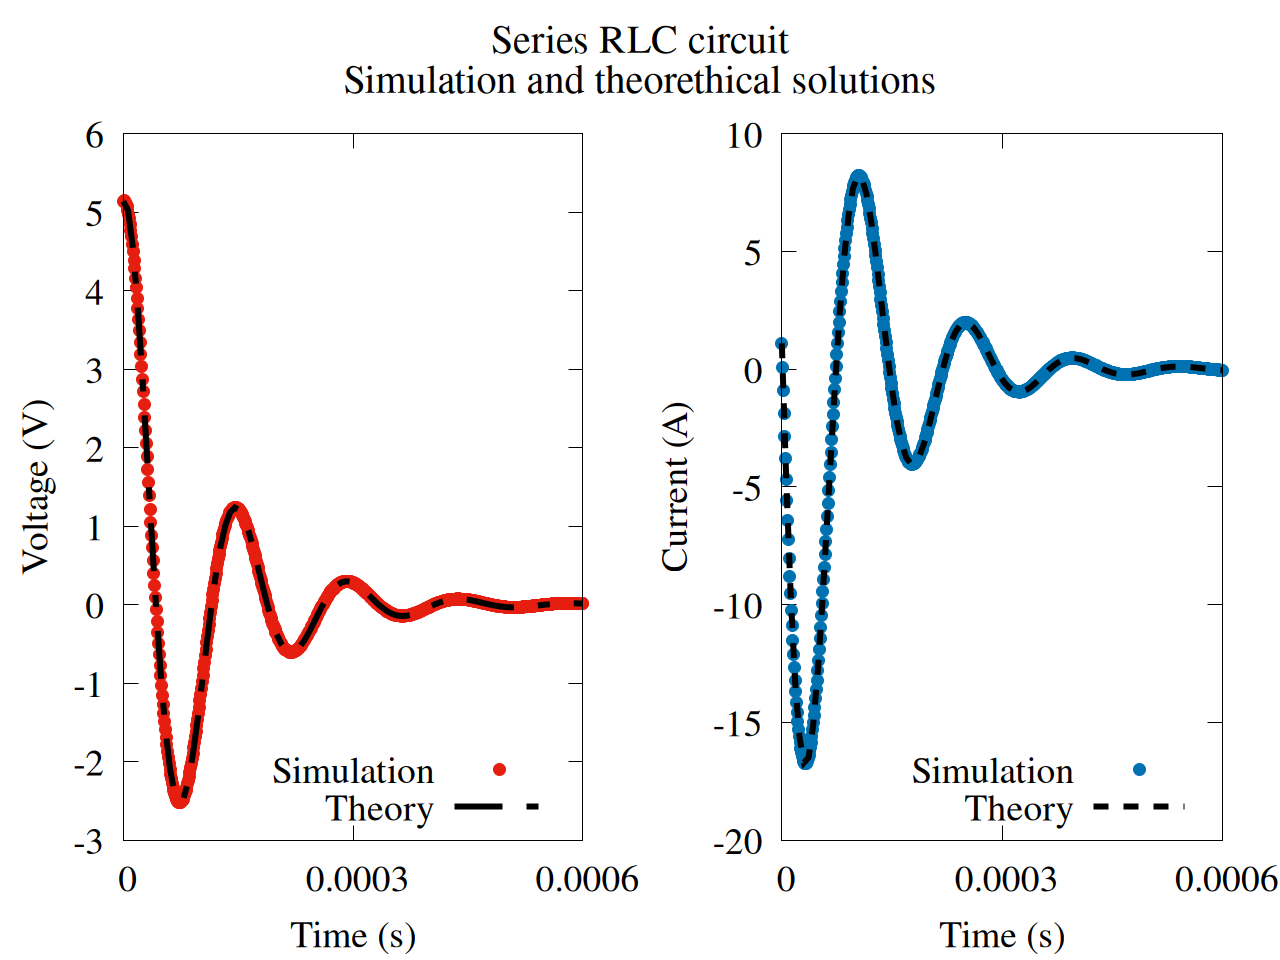
\includegraphics[width=0.9\textwidth]{figures/series_sim_vs_ana.png}
    \caption{Experimental data and fitting for the series RLC circuit.}
\label{fig:series_sva}
\end{figure}

\begin{figure}[ht]
    \centering
    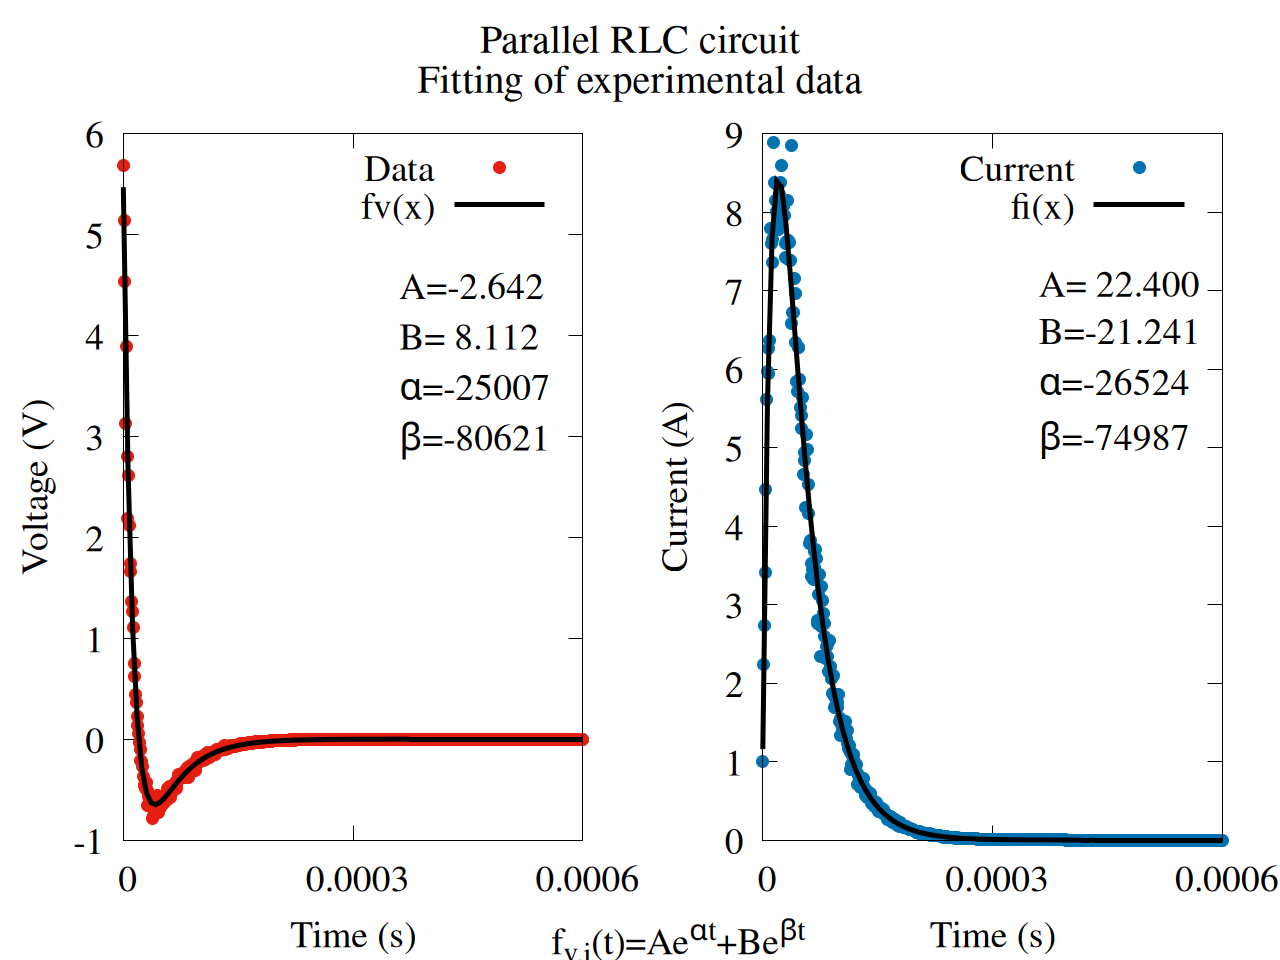
\includegraphics[width=0.9\textwidth]{figures/parallel_exp_vs_fitting.png}
    \caption{Experimental data and fitting for the parallel RLC circuit.}
    \label{fig:parallel_evf}
\end{figure}

\begin{figure}[ht]
    \centering
    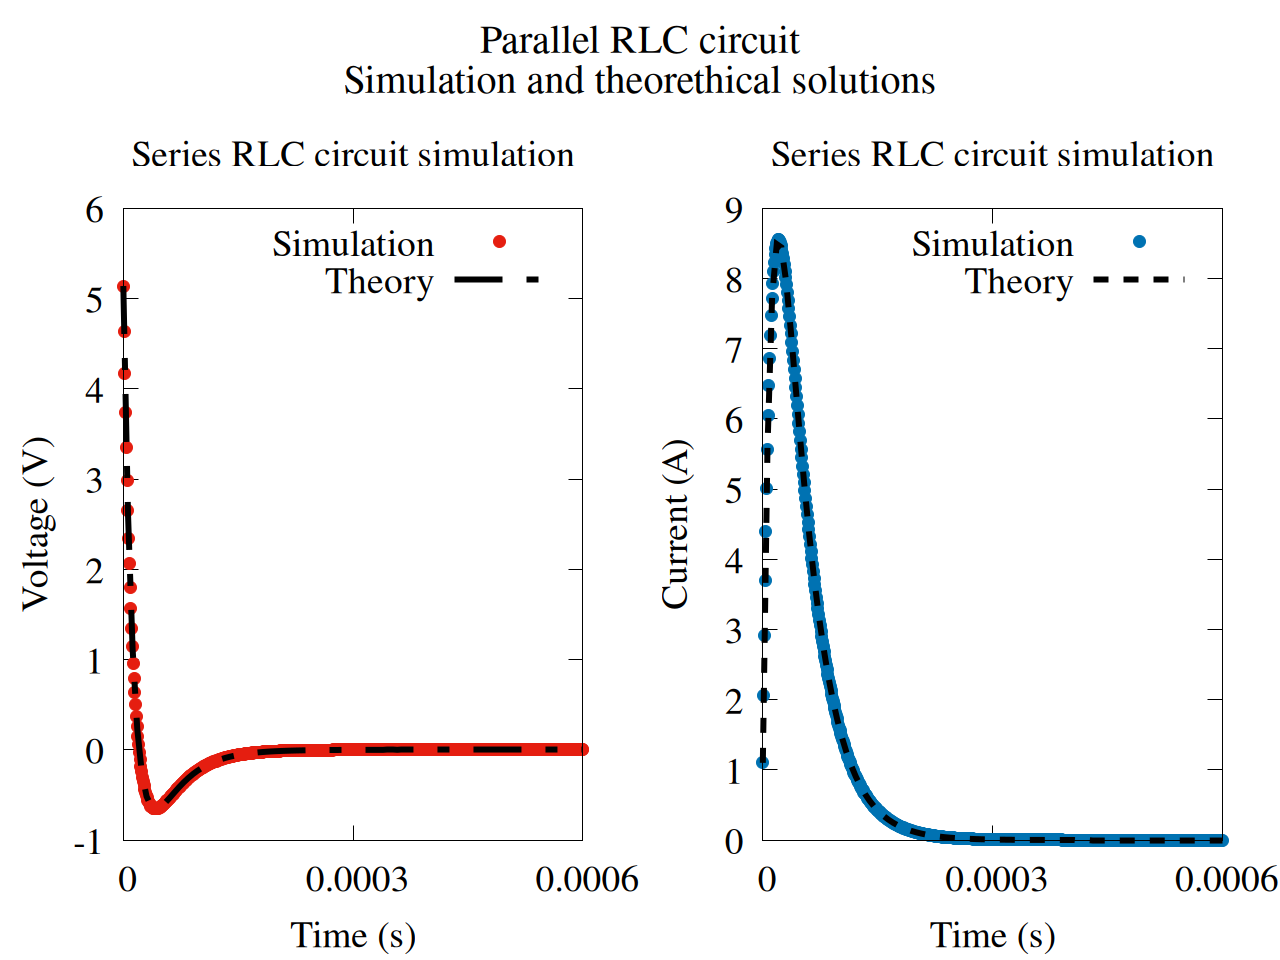
\includegraphics[width=0.9\textwidth]{figures/parallel_sim_vs_ana.png}
    \caption{Experimental data and fitting for the parallel RLC circuit.}
    \label{fig:parallel_sva}
\end{figure}




\section{Analysis}

%\begin{table}[!ht]
%    \centering
%    \resizebox{\textwidth}{!}{
%        \begin{tabular}{ccccc}
%        \toprule[3pt]
%       \multicolumn{1}{c}{\multirow{2}{*}{Type}} & \multicolumn{4}{c}{Parameter:}\\ 
%                                                  & $A$ & $\zeta $ & $\omega$ & $\phi$ \\
%        \midrule[2pt]
%           Experimental & 5.3217 & 9635.099 & 44318.060 & 1.303\\
%           Simulation   & 5.333 & 9803.920 & 43227.269 & 1.301\\
%           Analytical   & 5.333 & 9803.922 & 43227.2699 & 1.301\\
%        \midrule[2pt]
%           Error   & 0.512 & $9.273\times 10^{-2}$ & $0.208$ & $0.654$\\
%        \bottomrule[3pt]
%        \end{tabular}}
%    \caption{AAA}
%    \label{tab:series}
%\end{table}

\begin{table}[!ht]
    \centering
    \resizebox{\textwidth}{!}{
        \begin{tabular}{ccccc}
        \toprule[3pt]
       \multicolumn{1}{c}{\multirow{2}{*}{}} & \multicolumn{4}{c}{Parameter:}\\ 
                                                  & $A$ & $\alpha $ & $\omega$ & $\phi$ \\
        \midrule[2pt]
           Analytical reference   & 5.333 & 9803.922 & 43227.2699 & 1.301\\
        \midrule[2pt]
        Experimental error (\%)& $-0.206$ & $-1.722$ & $ 2.523$ & $ 0.173$ \\
        Simulation error (\%)& $4.947\times 10^{-12}$ & $-1.293\times 10^{-05}$ & $-1.570\times 10^{-06}$ & $8.738\times 10^{-12}$\\
        \bottomrule[3pt]
        \end{tabular}}
        \caption{Parameters of the analytical evolution of the voltage through a capacitor for the simple problem of series RLC circuit with values for the components of $R= 0.1\,\Omega$, $L= 5.1\,\mu H$, and $C= 9.98\,\mu F$; as well as the initial conditions $V_0= 5.14 V$ and $I_0= 1.1 A$. The circuit is clasiffied as underdamped, so its function is of the form $V(t)= Ae^{-\alpha t}\sin\qty(\omega t+\phi)$. The error generated by the parameters found using the Newton-Ramphson method for data fitting by non linear least squares of both datasets, obtained by experimental measurements and computer simulation, are also included. In both cases the resulting error is minimal.}
    \label{tab:series}
\end{table}
%
%Error simulation:
%A= 2.637889906509372e-13,      4.9465979984117304e-12
%decay= -0.0012672040284087416, -1.2925481089769163e-05
%omega= -0.0006786728190490976, -1.5700108302124718e-06
%phi= 1.1368683772161603e-13,   8.737592115756138e-12
%
%Error experimental:
%A= -0.01100128680505108,    -0.20629724976593036
%decay= -168.82239890795972, -1.721988468861189
%omega= 1090.7905668038657,   2.5233852827274896
%phi= 0.002246936091378604,   0.17269203251753995
%

\subsection{Parallel RLC circuit}
\begin{table}[!ht]
    \centering
    \resizebox{\textwidth}{!}{
        \begin{tabular}{ccccc}
        \toprule[3pt]
       \multicolumn{1}{c}{\multirow{2}{*}{}} & \multicolumn{4}{c}{Parameter:}\\ 
                                                  & $A$ & $\alpha $ & $B$ & $\beta$ \\
        \midrule[2pt]
           Analytical reference   & 23.309 & -26748.191 & -22.209 & -73452.209\\
        \midrule[2pt]
        Experimental error (\%) &$-3.899$ &$-0.835$ &$-4.358$ &$ 2.090$\\
        Simulation error (\%)& $ 0.541$ & $0.115$ & $0.567$ & $-0.314$\\
        \bottomrule[3pt]
        \end{tabular}}
        \caption{Parameters of the analytical evolution of the current through an inductor for the simple problem of a RLC circuit in parallel configuration, with values for the components of $R= 0.1\,\Omega$, $L= 5.1\,\mu H$, and $C= 9.98\,\mu F$; as well as the initial conditions $V_0= 5.14 V$ and $I_0= 1.1 A$. This is an overdamped circuit, so the function is of the form $I(t)=Ae^{\alpha}+Be^{\beta}$. The error generated by the parameters found using the Newton-Ramphson method for data fitting by non linear least squares of both datasets, obtained by experimental measurements and computer simulation, are also included. In both cases the resulting error is minimal.}
    \label{tab:parallel}
\end{table}



%%%%%%%%%%%%%%%%%%%%%%%%%%%%%
%% Conclusions
%%%%%%%%%%%%%%%%%%%%%%%%%%%%%
\section{Conclusion}
\noindent Conclusion .\cite{bobrow1983analisis}



%%%%%%%%%%%%%%%%%%%%%%%%%%%%%
%% References
%%%%%%%%%%%%%%%%%%%%%%%%%%%%%
\newpage\thispagestyle{empty}
\printbibliography\addcontentsline{toc}{section}{References}

%%%%%%%%%%%%%%%%%%%%%%%%%%%%%
%% Appendix (code)
%%%%%%%%%%%%%%%%%%%%%%%%%%%%%
\newpage\thispagestyle{empty}
\appendix
\section{Computational code (Python)}
%%\subsection{Circuit simulation}
%%\begin{code}\begin{lstlisting}[language=fortran,caption={Fortran code that solves the problem of a particle in a one dimentional infinite square well by the fine differences method. It solves for the functions, probability densities, orthogonality matrix, and a few statistically important integrals for the analisys of the first n energy levels. }, label=cd:fortran_gral]

program main
  use, intrinsic :: iso_fortran_env, only: sp=>real32, dp=>real64
  implicit none
  integer,parameter :: n=400, niveles=4
  real(dp),parameter :: x0=0, xf=1, fx0=1, fxf=1
  integer::i,j
  real(dp)::x,h,a(n),b(n),c(n),d(n),l(n),u(n),z(n),w(0:n+1),int_y
  real(dp)::fs(0:n+1,0:niveles),ort(niveles,niveles),dummy,dummy2,sigma

h=(xf-x0)/(n+1)
w(0)=fx0
w(n+1)=fxf
open(101,file="sh_n.dat")
open(100,file="sh.dat")
open(99,file="sh_n2.dat")

     do j=1,niveles
x=x0+h
a(1)=2+h*h*q(j,x) 
b(1)=-1+h*p(x)/2 
d(1)=-h*h*r(x)+(1+h*p(x)/2)*fx0 

!%##for ,nner inner point
do i = 2,n-1
        x=x0+h*i
        a(i)=2+h*h*q(j,x) 
        b(i)=-1+h*p(x)/2 
        c(i)=-1-h*p(x)/2 
        d(i)=-h*h*r(x)
enddo

!##for last inner point
x=xf-h
a(n)=2+h*h*q(j,x) 
c(n)=-1-h*p(x)/2 
d(n)=-h*h*r(x)+(1-h*p(x)/2)*fxf 
!##vectors a,b,c,d are populated

!#Solving the matrix
l(1)=a(1)
u(1)=b(1)/a(1)
z(1)=d(1)/l(1)

do i = 2,n-1
        l(i)=a(i)-c(i)*u(i-1)
        u(i)=b(i)/l(i)
        z(i)=(d(i)-c(i)*z(i-1))/l(i)
enddo

l(n)=a(n)-c(n)*u(n-1)
z(n)=(d(n)-c(n)*z(n-1))/l(n)

do i = 1,n
        w(i)=z(i)-fx0
enddo

do i = n-1,1,-1
        w(i)=z(i)-u(i)*w(i+1)
enddo

do i=0,n+1
        if (j==1) then
                fs(i,0)= x0+i*h
        endif
        write(100,*) fs(i,0), w(i)
enddo
write(100,*)  " "
int_y=simple_integral(h,w)
int_y=int_y

do i=0,n+1
        fs(i,j)=w(i)/sqrt(int_y)
        write(101,*) fs(i,0), fs(i,j)
        write(99,*) fs(i,0), fs(i,j)*fs(i,j)
enddo
write(101,*)  " "
write(99,*)  " "

        enddo
close(99)
close(100)
close(101)

do i=1,niveles
        do j=1,niveles
                ort(i,j)=double_integral(h,fs(:,i),fs(:,j))
        enddo
enddo

open(102,file="sh.ortm")
do i=1,niveles
        write(102,*) ort(:,i)
enddo
close(102)

open(103,file="sh.stat")
do i=1,niveles
        dummy=expx(h,fs(:,0),fs(:,i))
        dummy2=expx2(h,fs(:,0),fs(:,i))
        sigma=sqrt(dummy2-dummy*dummy)
        write(103,*) "       <x> for level",i," is ", dummy
        write(103,*) "      <x2> for level",i," is ", dummy2
        write(103,*) "<x2>-<x>^2 for level",i," is ", dummy2-dummy*dummy
        write(103,*) "        SD for level",i," is ", sigma
        write(103,*) "Probability to to find electron between x+sigma and x-sigma"
        write(103,*)  prob(h,fs(:,0),fs(:,i), dummy-sigma , dummy+sigma)
        write(103,*) "Probability to to find electron between 0.45 and 0.55"
        write(103,*)  prob(h,fs(:,0),fs(:,i), 0.45D0, 0.55D0)
        write(103,*) "Probability to to find electron on the left side"
        write(103,*)  prob(h,fs(:,0),fs(:,i), 0D0, 0.5D0)
        write(103,*) "Probability to to find electron on the first quarter"
        write(103,*)  prob(h,fs(:,0),fs(:,i), 0D0, 0.25D0)
        write(103,*) " "
enddo
close(103)


contains
real(dp) function p(r) result(f)
  implicit none
  real(dp), intent(in) :: r
    f = 0D0
end function p

real(dp) function q(well_n, r) result(E)
  implicit none
  real(dp), intent(in) :: r
  integer, intent(in) :: well_n
  real(dp), parameter:: m=1D0,  pi=3.14159265
    E =-(well_n*pi*well_n*pi)
end function q

real(dp) function r(x) result(f)
  implicit none
  real(dp), intent(in) :: x
    f = 0D0
end function r

real(dp) function simple_integral(h,y) result(f)
  real(dp), intent(in) :: h, y(0:)
  integer ::i
    f=y(0)*y(0)
    do i=1, (size(y)-1)/2
         f=f+4*y(2*i-1)*y(2*i-1)
    enddo
    do i=2, (size(y)-1)/2-1
         f=f+2*y(2*i)*y(2*i)
    enddo
    f=f+y(size(y)-1)*y(size(y)-1)
    f=f*h/3
end function simple_integral

real(dp) function double_integral(h,y,w) result(f)
  real(dp), intent(in) :: h, y(0:), w(0:)
  integer ::i
    f=w(0)*y(0)
    do i=1, (size(y)-1)/2
         f=f+4*w(2*i-1)*y(2*i-1)
    enddo
    do i=2, (size(y)-1)/2-1
         f=f+2*w(2*i)*y(2*i)
    enddo
    f=f+w(size(y)-1)*y(size(y)-1)
    f=f*h/3
end function double_integral

real(dp) function prob(h,x, w,a,b) result(f)
  real(dp), intent(in) :: h, x(0:), w(0:), a, b
  integer :: xa(1), xb(1)
  integer ::i , ia , ib
    xa=minloc(abs(x-a))
    xb=minloc(abs(x-b))
    ia=xa(1)
    ib=xb(1)
    if (MOD(ib-ia,2)==0) then
        f=w(ia)*w(ia)
        do i=ia+1, ib-1, 2
             f=f+4*w(i)*w(i)
        enddo
        do i=ia+2, ib-1, 2
             f=f+2*w(i)*w(i)
        enddo
        f=f+w(ib)*w(ib)
        f=f*h/3
    else 
        ib=ib+1
        f=w(ia)*w(ia)
        do i=ia+1, ib-1, 2
             f=f+4*w(i)*w(i)
        enddo
        do i=ia+2, ib-1, 2
             f=f+2*w(i)*w(i)
        enddo
        f=f+w(ib)*w(ib)
        f=f*h/3
    endif
end function 

real(dp) function expx(h,x,w) result(f)
  real(dp), intent(in) :: h, x(0:), w(0:)
  integer ::i
    f=x(0)*w(0)*w(0)
    do i=1, (size(w)-1)/2
        f=f+4*x(2*i-1)*w(2*i-1)*w(2*i-1)
    enddo
    do i=2, (size(w)-1)/2-1
        f=f+2*w(2*i)*w(2*i)*x(2*i)
    enddo
    f=f+x(size(x)-1)*w(size(w)-1)*w(size(w)-1)
    f=f*h/3
end function 
        
real(dp) function expx2(h,x,w) result(f)
  real(dp), intent(in) :: h, x(0:), w(0:)
  integer ::i
    f=x(0)*x(0)*w(0)*w(0)
    do i=1, (size(w)-1)/2
        f=f+4*x(2*i-1)*x(2*i-1)*w(2*i-1)*w(2*i-1)
    enddo
    do i=2, (size(w)-1)/2-1
        f=f+2*w(2*i)*w(2*i)*x(2*i)*x(2*i)
    enddo
    f=f+x(size(x)-1)*x(size(x)-1)*w(size(w)-1)*w(size(w)-1)
    f=f*h/3
end function 

end program



\end{lstlisting}
\end{code}

%%\subsection{Data fitting}
%%\begin{code}\begin{lstlisting}[language=python,caption={Python code that approximated the function of the voltage and current for a discharging RLC series circuit. }, label=cd:fortran_gral]
import numpy as np
import matplotlib.pyplot as plt

# Define the decaying sine function
def decaying_sine(x, A, omega, phi, decay):
    return A * np.exp(-decay * x) * np.sin(omega * x + phi)

# Define the Jacobian of the decaying sine function
def Jacobian(f, x, A, omega, phi, decay, eps):
    grad_a = ( f(x, A-2*eps, omega, phi, decay)/12 - f(x, A-eps, omega, phi, decay)*2/3 + f(x, A+eps, omega, phi, decay)*2/3 - f(x, A+2*eps, omega, phi, decay)/12)/(eps)
    grad_o = ( f(x, A, omega-2*eps, phi, decay)/12 - f(x, A, omega-eps, phi, decay)*2/3 + f(x, A, omega+eps, phi, decay)*2/3 - f(x, A, omega+2*eps, phi, decay)/12)/(eps)
    grad_p = ( f(x, A, omega, phi-2*eps, decay)/12 - f(x, A, omega, phi-eps, decay)*2/3 + f(x, A, omega, phi+eps, decay)*2/3 - f(x, A, omega, phi+2*eps, decay)/12)/(eps)
    grad_d = ( f(x, A, omega, phi, decay-2*eps)/12 - f(x, A, omega, phi, decay-eps)*2/3 + f(x, A, omega, phi, decay+eps)*2/3 - f(x, A, omega, phi, decay+2*eps)/12)/(eps)
    return np.column_stack([grad_a, grad_o, grad_p, grad_d])

def Gauss_Newton(f, x, y, A0, o0, p0, d0, eps, maxit, tol):
    old = new = np.array([A0, o0, p0, d0])
    for itr in range(maxit):
        old = new
        J = Jacobian(f, x, old[0], old[1], old[2], old[3], eps)
        dy = y - f(x, old[0], old[1], old[2], old[3])
        new = old + np.linalg.inv(J.T@J)@J.T@dy
        if np.linalg.norm(old-new) < tol:
            break
        return new

# Load the dataset
data = np.loadtxt('cap_test.dat')  # replace 'data.txt' with the actual filename

# Extract the x and y values from the dataset
x = data[:, 0]
y = data[:, 1]

# Guess initial values for the parameters
A_guess = np.max(y) - np.min(y)
omega_guess = 14
phi_guess = 0.3
decay_guess = 6.5

A_fit, omega_fit, phi_fit, decay_fit = Gauss_Newton(decaying_sine, x, y, A_guess, omega_guess, phi_guess, decay_guess, 1e-15, 5000, 1e-20)

yhat= decaying_sine(x, A_fit, omega_fit, phi_fit, decay_fit)

# Print the results
print(f"A: {A_fit}")
print(f"Frequency: {omega_fit / (2 * np.pi)}")
print(f"Decaying constant: {decay_fit}")
print(f"phi constant: {phi_fit}")
print(f"wd: {(omega_fit*omega_fit+ decay_fit*decay_fit )**0.5}")

plt.scatter(x,y)
plt.plot(x,yhat)
plt.show()

\end{lstlisting}
\end{code}

\end{document}
